%%Énoncé
Citez au moins quatre implémentations différentes d'un dictionnaire.
Précisez, dans chaque cas, quelles sont les propriétés principales de ces implémentations.
Dans quel(s) cas s'avèrent-elles intéressantes ?
Quelles sont les complexités calculatoires de leur principales méthodes ?
Une \textit{Skip List} constitue-t-elle une implémentation possible d'un dictionnaire non ordonné ?
Pourquoi ? \textit{(Tanguy)}
\\

%%Réponse
Un dictionnaire permet de stocker des paires <clé, valeur> appelées des entrées.
Contrairement aux \textit{Map's}, qui n'accepte que des clés uniques, un dictionnaire autorise plusieurs entrées avec la même clé.
Dans les quatre implémentations ci-dessous, nous augmentons le type des entrées qui seront stockées afin qu'elles possèdent une variable \textit{position}. Cette variable devra à tout moment indiquer quelle est la position de l'entrée dans la structure de données. Ce mécanisme est détaillé dans DSAJ-5 section 4.8.2.
\\
\textit{Citez au moins quatre implémentations différentes d'un dictionnaire.}
\begin{enumerate}
	\item Liste non-ordonnée.\\
			Dans le cas d'une liste non-ordonnée, nous pouvons utiliser la méthode \textit{remove(entry)} comme suit : \textit{list.remove(entry.location())} qui s'exécutera en $\Theta(1)$.
			Cette implémentation est intéressante lorsqu'on devra à la fois ajouter et retirer de nombreuses entrées.
	\item Hashtable.\\
			Nous avons ici une table hachée avec un \textit{"bucket array"},  en français un \textit{tableau de seaux} littéralement. l'implémentation utilise la fonction de hachage \textit{h} et utilise des chaines séparées pour gérer les collisions. Cette explication est représentée schématiquement sur la figure \ref{fig:hashtable}\footnote{Source wikipédia: \url{https://en.wikipedia.org/wiki/Hash_table}}. Lors de l'appel à la méthode \textit{remove(entry)}, la méthode de hachage est utilisée pour accéder au bon emplacement dans le tableau (au bon \textit{"bucket"}). Avec une méthode de hachage efficace, les collisions sont rares et chaque bucket ne contiendra que 1 ou 0 élément mais rarement plus. Si il y en a plus, la variable \textit{location} permettra de déterminer la position de l'élément recherché. La méthode \textit{hachtable.remove(entry.location())} s'exécutera donc en $\Theta(1)$.
			Cette implémentation sera intéressante quand on aura très peu d'entrées avec la même clé (car il y aura alors peu de collision).
	\item Table ordonnée de recherche.\
			Dans une table ordonnée de recherche, la variable \textit{location} est un entier indiquant l'index de l'élément dans la table.
			La méthode \textit{table.remove(entry.location())} s'exécutera en $\Theta(n)$ car il faudra déplacer $n$ éléments de la liste pour la maintenir ordonnée. Le meilleur des cas étant le cas où \textit{entry} est la dernière entrée de la liste et le pire des cas où \textit{entry} est la première entrée de la liste.
			Cette implémentation est intéressante si l'on ajoute les entrées de manière ordonnée puis que l'on doit faire de nombreuses recherches dessus.
	\item Skip List.\\
			Une Skip List est une liste de listes ($S_0$, $S_1$, $...$, $S_h$) où $h$ est la taille de la Skip List.
			Chaque sous-liste $S_i$ contient les éléments $+\infty$ et $-\infty$ ainsi qu'un sous-ensemble des éléments de $S_{i-1}$.
			Ainsi, la liste $S_0$ contient tous les éléments plus $+\infty$ et $-\infty$. Ces éléments sont stockés dans l'ordre croissant. $-\infty$ étant plus petit que toutes entrées pouvant être insérée dans la liste, il sera toujours le premier élément et $+\infty$, de manière équivalente, sera toujours le dernier élément.
			Pour construire la sous-liste $S_i$, après avoir ajouté les éléments $+\infty$ et $-\infty$, les éléments de $S_{i-1}$ sont parcourus un à un et chacun d'eux à une probabilité de 0,5 d'être ajouté dans $S_i$. Si $S_0$ possède $n$ éléments, on s'attend à ce que $S_1$ en possède $n/2$, $S_2$ $n/4$ et $S_i$ $n/2^i$. On s'attend donc aussi à ce que la hauteur $h$ de la skip list soit égale à $\\log (n)$
			La figure \ref{fig:skiplist} représente une Skip List de hauteur 5 contenant 10 éléments\footnote{Source: DSAJ-5, Figure 9.9, page 412}.
			Nous pouvons voir une Skip List comme étant une structure à deux dimensions de positions agencées horizontalement en niveaux et verticalement en tours. Chaque niveau est une liste $S_i$ et chaque tour contient les positions référençant la même entrée à travers les différentes listes.
			Les Skip List permette d'effectuer des recherches grâce à une méthode appelée SkipSearch. Cette méthode est détaillée dans DSAJ-5 page 413. L'idée générale est de rechercher une entrée ayant pour clé $k$ en partant du haut de la liste (l'élément le plus à droite de la liste la plus haute, c'est-à-dire toujours $-\infty$). Ensuite, on parcourt le niveau courant vers la droite tant que la valeur de la clé de l'élément suivant est $< k$. Ce cas existera toujours car chaque niveau contient l'élément $+\infty$. Ensuite on navigue vers le bas dans la tour et on recommence la méthode jusqu'à atteindre $S_0$.
			Les méthodes permettant d'insérer, retirer et rechercher une entrée dans une Skip List s'exécuteront en moyenne en $\Theta(\log(n))$.
			Cette implémentation est intéressante dans le cas où on ferait de nombreuses opérations (insertion, recherche, suppression).
			\\
			\textit{Une \textit{Skip List} constitue-t-elle une implémentation possible d'un dictionnaire non ordonné ? Pourquoi ?}
			\\
			Il est possible d'implémenter un dictionnaire en utilisant une Skip List. La varialbe \textit{location} de chaque entrée sera égale à la position de l'entrée dans le bas de la liste (en $S_0$).
\end{enumerate}

\begin{figure}
	\centering
	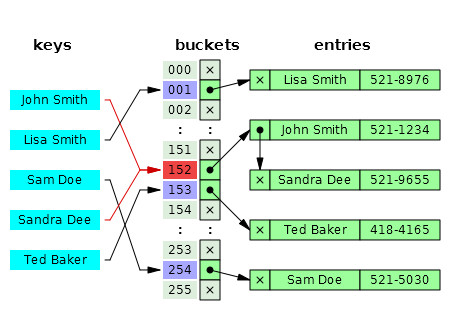
\includegraphics[width=\textwidth/3*2]{hachtable.jpg}
	\caption{Hachtable with collision resolve by separate chaining.}
	\label{fig:hashtable}
\end{figure}

\begin{figure}
	\centering
	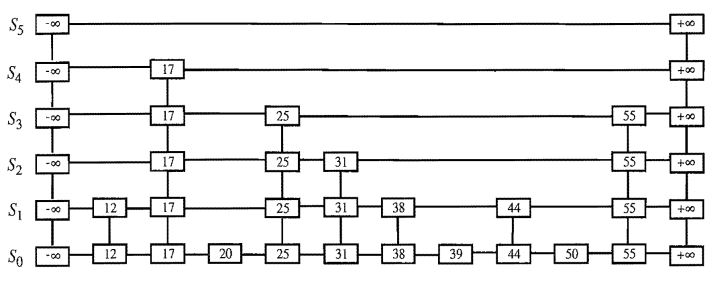
\includegraphics[width=\textwidth/3*2]{skiplist.jpg}
	\caption{Example of skip list storing 10 entries.}
	\label{fig:skiplist}
\end{figure}